\documentclass{beamer}
\usepackage[italian]{babel}
\usetheme{Berkeley}
\usepackage{graphicx}
\usepackage{booktabs}

\title{PineSU - Workflow}
\subtitle{Sviluppo di un'applicazione distribuita su Blockchain Ethereum}
\author{Paolo Speziali}
\institute{Università degli Studi di Perugia - Dipartimento di Ingegneria\\[\medskipamount]
      
\includegraphics[width=0.15\textwidth,height=0.15\textwidth]{figures/logo_unipg.png}%
 }
\logo{
\includegraphics[height=1cm]{figures/favicon.png}}
\date{A.A. 2020/2021}

\begin{document}
\begin{frame}
	\titlepage % beamer's \maketitle
\end{frame}
\section{Operazioni}
\begin{frame}
	\frametitle{Operazioni eseguibili}
	Nell'applicativo è possibile eseguire le seguenti operazioni:
	\begin{enumerate}
		\item Creazione di una Storage Unit (SU)
		\item Registrazione di una o più SU nella blockchain Ethereum
		\item Esportazione di sottoinsiemi di file da una SU
		\item Controllo d'integrità su una SU
		\item Controllo d'integrità di singoli file esportati da altre SU
	\end{enumerate}
	Oltre a poter eseguire tutti i comandi di Git. Vedremo ora questi comandi uno per uno utilizzando una directory campione da trasformare in Storage Unit.
\end{frame}
\begin{frame}
	\frametitle{Directory campione}
	Utilizzeremo come directory campione per mostrare l'evoluzione della Storage Unit una cartella chiamata \emph{sample} con la seguente struttura (dove \emph{first} e \emph{second} sono sottodirectory di \emph{sample} e \emph{third} è sottodirectory di \emph{second}):
	\smallskip
	\begin{figure}
		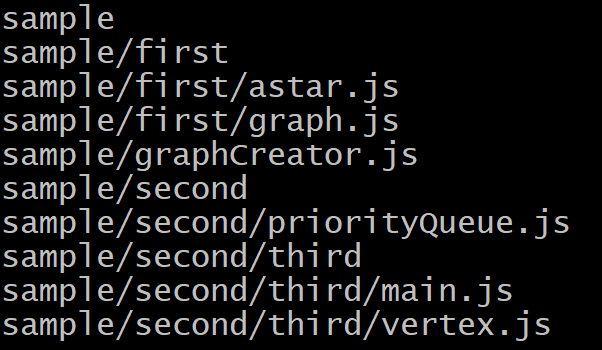
\includegraphics[width=0.80\textwidth]{figures/sample1.png}
	\end{figure}
\end{frame}
\section{Creazione}
\begin{frame}
	\frametitle{Creazione di una SU}
	La creazione di una Storage Unit è in realtà un'operazione che comprende sia la trasformazione in una Git Repository della directory, sia il calcolo degli hash che serviranno poi per registrare la nostra SU nella blockchain.
	\\

	Le informazioni della nostra SU sono conservate nel file \textbf{.pinesu.json} nella root della directory, la presenza di questo file indica al programma che la directory è già una SU.
	\\

	La creazione potrebbe eventualmente venire suddivisa in due azioni diverse, ma a quel punto la prima fase si limiterebbe ad eseguire un comando "git init" sulla directory, comando che potrebbe non essere necessario.
\end{frame}
\begin{frame}
	\frametitle{Creazione di una SU}
	Tuttavia, per come il programma è ora strutturato, la creazione della Storage Unit la rende pronta per essere registrata (eventualmente insieme ad altre) nella blockchain.
	\\

	Andiamo quindi a vedere quali sono le operazioni che avvengono in questa fase e come la nostra directory \emph{sample} cambia.
\end{frame}
\begin{frame}
	\frametitle{Creazione di una SU}
	\begin{itemize}
		\item Controlla se nella directory è già presente \textbf{.pinesu.json}, in caso negativo continua;
		\item Permette all'utente di selezionare dei file da ignorare da tutto il processo, ciò produce un file \textbf{.gitignore};
		\item Aggiunge tutti i file della directory nella Git Staging Area e crea un commit fantoccio;
		\item Recupera la lista dei file dal commit;
		\item Calcola gli hash di tutti i file (non directory);
		\item Calcola gli hash delle directory creando dei Merkle Tree con gli hash del loro contenuto e usa l'hash della radice come hash della directory, ciò avviene tramite un approccio bottom-up: calcola prima gli hash delle directory senza file al loro interno;
	\end{itemize}
\end{frame}
\begin{frame}
	\frametitle{Creazione di una SU}
	\begin{itemize}
		\item Calcola l'hash della SU creando un Merkle Tree con tutti gli hash dei file e delle directory in essa contenute e ne prende la radice;
		\item Viene generato il file \textbf{.pinesu.json} con al suo interno nome, descrizione, visibilità, data, hash dell'utente, hash della SU, lista dei file e delle sottodirectory con hash associati;
		\item Aggiunge tutti i file della directory nella Git Staging Area e crea un commit fantoccio;
		\item Aggiungo il percorso di questa SU con il suo hash alla lista della SU generate dall'utente (memorizzata nella cartella d'installazione del programma);
		\item Viene annullato il commit fantoccio e creato uno effettivo con informazioni consistenti e aggiunto \textbf{.pinesu.json};
	\end{itemize}
\end{frame}
\begin{frame}
	\frametitle{Creazione di una SU - Risultato}
	L'operazione di creazione ha prodotto nella cartella \emph{sample}, ovviamente, una sottocartella \emph{.git} e il file \textbf{.pinesu.json}. L'ordine di calcolo degli hash è stato questo:
	\newcounter{currentenumi}
	\begin{enumerate}
		\item sample/first/astar.js
		\item sample/first/graph.js
		\item sample/graphCreator.js
		\item sample/second/priorityQueue.js
		\item sample/second/third/main.js
		\item sample/second/third/vertex.js
		\setcounter{currentenumi}{\theenumi}
	\end{enumerate}
\end{frame}
\begin{frame}
	\frametitle{Creazione di una SU - Risultato}
	\begin{enumerate}
		\setcounter{enumi}{\thecurrentenumi}
		\item sample/first (tramite MT dei due file da lui contenuti)
		\item sample/second/third (tramite MT dei due file da lui contenuti)
		\item sample/second (tramite MT del file e della sottodirectory \emph{third} da lui contenuti)
		\item sample (tramite MT degli hash dei tutti i file e le directory appena visti)
	\end{enumerate}
	Si può quindi facilmente osservare come questa tecnica di calcolo di hash bottom-up viene messa in atto calcolando prima i file effettivi, poi le directory senza sottodirectory e infine tutto il resto delle directory.
\end{frame}
\section{Registrazione}
\begin{frame}
	\frametitle{Registrazione di una o più SU nella blockchain}
	In questa fase all'utente viene data la libertà di scegliere se registrare con un unico hash una o più SU insieme, poiché il workflow è praticamente identico andrò a separare i punti esclusivi ad una registrazione “multipla” scrivendoli in color oliva:
	\begin{itemize}
		\item Mostra la selezione multipla della SU registrate dall'utente per permettere di registrarne una sola o più in una volta;
		\item \textcolor{olive}{Per ogni Storage Unit selezionata} creo nella root della SU il file \textbf{.registration.json} che contiene l'hash della directory, l'hash che verrà salvato nella blockchain (stesso valore se registriamo una sola SU, \textcolor{olive}{valore della root del MT di tutti gli hash delle SU selezionate se la registrazione è multipla})
	\end{itemize}
\end{frame}
\begin{frame}
	\frametitle{Excursus sulle Applicazioni Distribuite}
	\begin{figure}
		
\includegraphics[width=0.90\textwidth]{figures/truffle.png}
	\end{figure}
	\bigskip
	Su tale rete è possibile mettere a disposizione delle applicazioni che chiunque può utilizzare dietro pagamento di una piccola commissione. Queste applicazioni sono realizzabili dagli sviluppatori interessati tramite vari framework e suite di applicativi, il più celebre è \textbf{Truffle}.
\end{frame}
\begin{frame}
	\frametitle{Excursus su Git}
	Git è un software che permette in maniera semplice di gestire insiemi di file tramite un sistema di controllo di versione, una grande risorsa per gli sviluppatori che devono contribuire in maniera condivisa ad uno stesso progetto o che devono tenere sotto controllo i vari cambiamenti che sono stati apportati ai vari file e documenti.
	\begin{figure}
		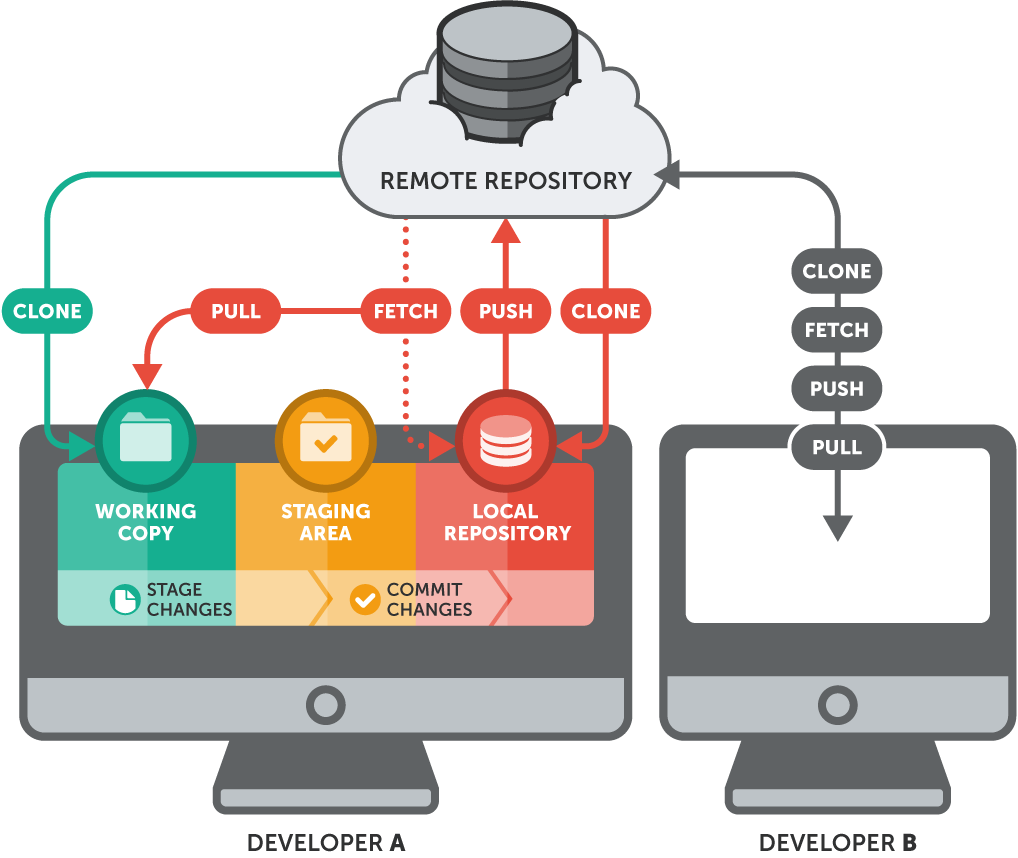
\includegraphics[width=0.45\textwidth]{figures/git2.png}
	\end{figure}
\end{frame}
\begin{frame}
	\frametitle{Excursus sulle funzioni di hashing}
	Le funzioni di hashing sono funzioni non invertibili che permettono di associare in maniera univoca (o quasi) stringhe di caratteri (e quindi anche documenti di varia natura tradotti in stringhe) a delle stringhe alfanumeriche di lunghezza fissa.
	\bigskip
	\begin{figure}
		
\includegraphics[width=0.85\textwidth]{figures/hashing.jpg}
	\end{figure}
\end{frame}
\section{Progettazione}
\begin{frame}
	\frametitle{Fase 3: Progettazione - Prima stesura}
	\begin{columns}
		\column{0.5\textwidth}
			La stesura iniziale è stata svolta dal professore che mi ha quindi fornito una linea guida da cui poter prendere spunto per poter realizzare il progetto dopo aver concordato sulle sue funzionalità, tale architettura è stata tuttavia modificata abbastanza in quanto le tecnologie utilizzate sono ancora troppo sperimentali e non offrono gli strumenti per potere essere adattati ad una struttura del genere.
		\column{0.5\textwidth}
		\begin{figure}
			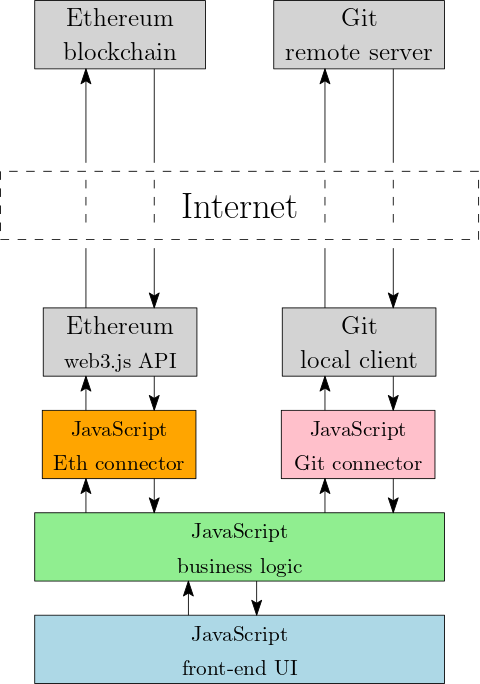
\includegraphics[width=0.88\textwidth]{figures/architecture1.png}
		\end{figure}
	\end{columns}
\end{frame}
\begin{frame}
	\frametitle{Fase 3: Progettazione - Seconda stesura}
	\begin{columns}
		\column{0.5\textwidth}
			\begin{figure}
				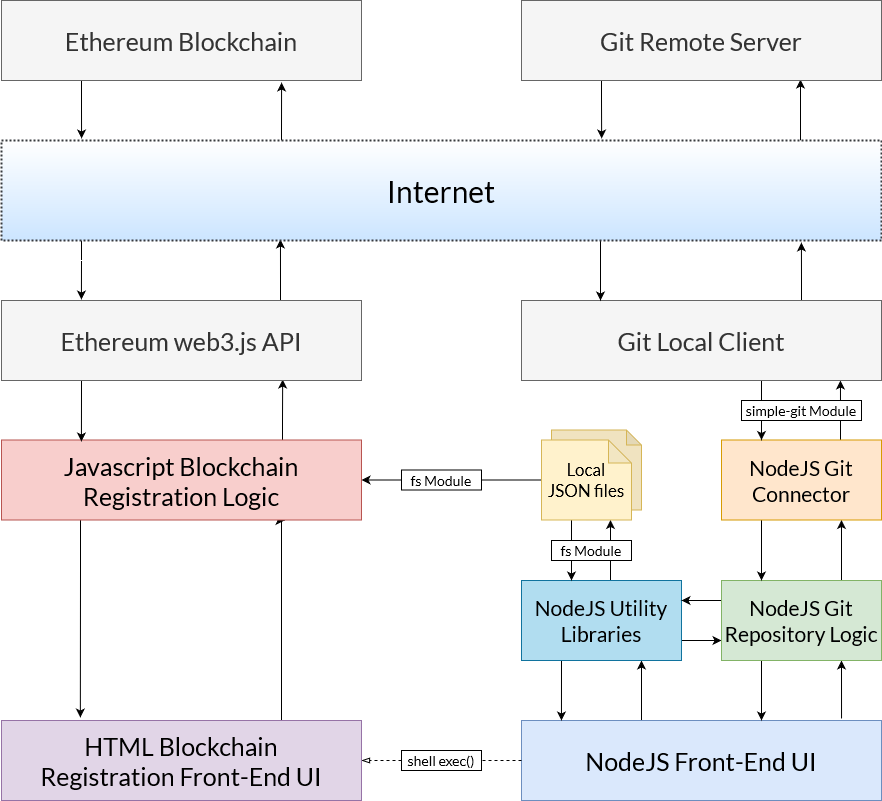
\includegraphics[width=1\textwidth, height=1.05\textwidth]{figures/architecture2.png}
			\end{figure}
		\column{0.5\textwidth}
		Il Front-End in NodeJS che comunica con una parte logica è stato mantenuto, sono stati però introdotti alcuni moduli Utility che vengono utilizzati da entrambe le componenti.

		La connessione alla Blockchain avviene attraverso l’avvio di un Web Server apposito e l’apertura di una scheda del browser, l’interazione da parte dell’utente deve avvenire tramite l’add-on \textbf{Metamask}.
	\end{columns}
\end{frame}
\section{Apprendimento}
\begin{frame}
	\frametitle{Fase 4: Apprendimento}
	In concomitanza con la fase di progettazione è stato necessario l’apprendimento di alcune tecnologie in modo da poter imparare le loro modalità di utilizzo e poter effettuare la seconda stesura dello schema progettuale.

	Oltre ai già citati Truffle Suite e Metamask, abbastanza intuitivi nell'utilizzo, le tecnologie che seguono sono quelle che hanno occupato la maggior parte di questa fase.
	\begin{figure}
		
\includegraphics[width=0.50\textwidth]{figures/metamask.png}
	\end{figure}
\end{frame}
\begin{frame}
	\frametitle{Fase 4: Apprendimento - Solidity}
	\begin{columns}
		\column{0.5\textwidth}
		Per l’apprendimento della sintassi e delle peculiarità del linguaggio da utilizzare per scrivere DAPP per la Blockchain Ethereum mi sono avvalso della documentazione ufficiale e del tutorial interattivo \textbf{CryptoZombies}.	
		\column{0.5\textwidth}
		\begin{figure}
			
\includegraphics[width=0.30\textwidth]{figures/solidity.png}
		\end{figure}
		\begin{figure}
			
\includegraphics[width=0.40\textwidth]{figures/zombie.png}
		\end{figure}
	\end{columns}
\end{frame}
\begin{frame}
	\frametitle{Fase 4: Apprendimento - Javascript Asynchronous Programming}	
	\begin{figure}
		
\includegraphics[width=0.65\textwidth]{figures/async.jpg}
	\end{figure}
	L’utilizzo di alcuni moduli all’interno dell’applicazione ha richiesto che io spendessi diverso tempo ad imparare le tecniche di programmazione asincrona di Javascript in quanto lo scorretto utilizzo delle keyword async e await sono state fonte di svariati problemi nella prima fase della stesura del codice.
\end{frame}
\begin{frame}
	\frametitle{Fase 4: Apprendimento - Modulo Merkle Tree}
	\begin{columns}
		\column{0.5\textwidth}
		La necessità di dover calcolare una singola stringa Hash per una moltitudine di file ha portato il professore a proporre l’utilizzo di questa struttura, è stato quindi necessario da parte mia non solo comprenderne bene il funzionamento ma anche essere in grado di poter utilizzare al meglio i moduli che fornivano metodi per lavorare con questi particolari alberi.
		\column{0.5\textwidth}
		\begin{figure}
			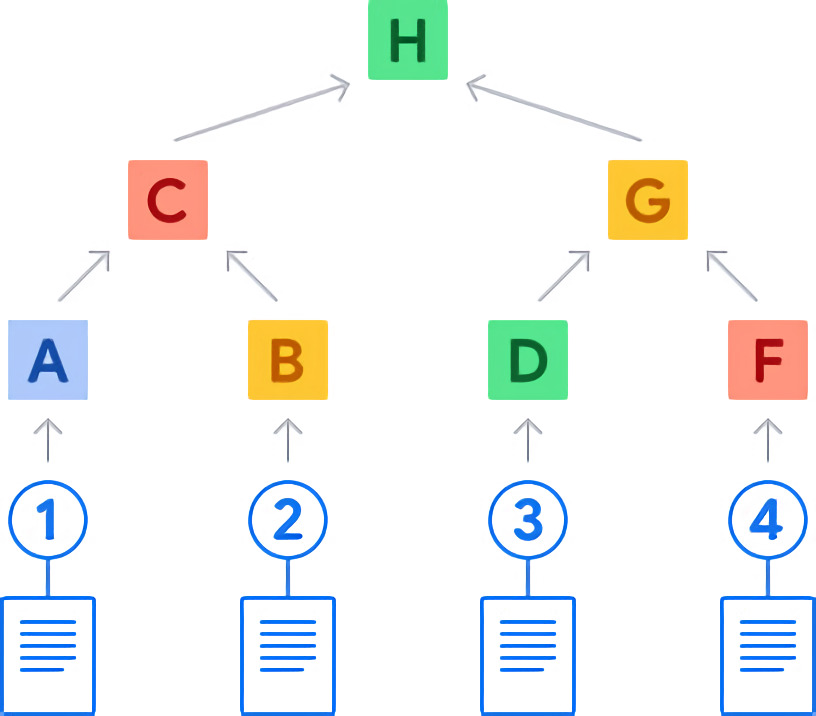
\includegraphics[width=0.88\textwidth]{figures/merkle-tree.jpg}
		\end{figure}
	\end{columns}
\end{frame}
\begin{frame}
	\frametitle{Fase 4: Apprendimento - Modulo InquirerJS}
	\begin{columns}
		\column{0.5\textwidth}
			\begin{figure}
				
\includegraphics[width=1\textwidth]{figures/inquirer.png}
			\end{figure}
		\column{0.5\textwidth}
		Anziché realizzare un Front-End dotato di GUI, ho preferito optare per una interfaccia testuale. Tuttavia, non volendo rinunciare all’immediatezza e la semplicità che un approccio grafico e user-friendly poteva portare al progetto ho imparato ad utilizzare il modulo di InquirerJS, il quale consente di realizzare menù a scelta singola, multipla e libera in tutta comodità.
	\end{columns}
\end{frame}
\section{Implementa -zione}
\begin{frame}
	\frametitle{Fase 5: Implementazione}
	La fase di implementazione è divisibile in tre macro-sezioni:
	\begin{enumerate}
		\item Creazione delle librerie di utility e dei moduli di interfacciamento con Git
  		\item Creazione della CLI e del flow di interazione con le librerie e la logica di Git
  		\item Creazione del modulo di interrogazione e registrazione per la Blockchain
	\end{enumerate}
\end{frame}
\begin{frame}
	\frametitle{Creazione delle librerie di utility e dei moduli di interfacciamento con Git}
	La prima stesura di codice è avvenuta nella creazione della classe “connettore” per Git con il modulo “simple-git” e del relativo modulo Logic il quale richiama le sue funzioni a seconda della necessità della CLI.
\end{frame}
\begin{frame}
	\frametitle{Creazione delle librerie di utility e dei moduli di interfacciamento con Git}
	In concomitanza ho scritto i moduli del package “lib”:
	\begin{itemize}
		\item files: Lettura e scrittura di file JSON in cui conservare le informazioni riguardanti la Storage Unit o l’utente che sta utilizzando l’applicativo;
		\item inquirer: Contiene tutte le scelte che vengono poi presentate all’utente nella CLI;
		\item treelist: Si occupa di effettuare tutte le operazioni riguardanti l’hashing di file, l’assegnazione di hash alle subdirectories e la creazione e gestione di Merkle Tree.
	\end{itemize}
\end{frame}
\begin{frame}
	\frametitle{Creazione della CLI e del flow di interazione con le librerie e la logica di Git}
	Ho proseguito andando a creare l’effettivo workflow del programma richiamando le scelte dal modulo inquirer e funzioni differenti in base alle selezioni dell’utente.	
\end{frame}
\begin{frame}
	\frametitle{Creazione della CLI e del flow di interazione con le librerie e la logica di Git - Workflow}
	\begin{figure}
		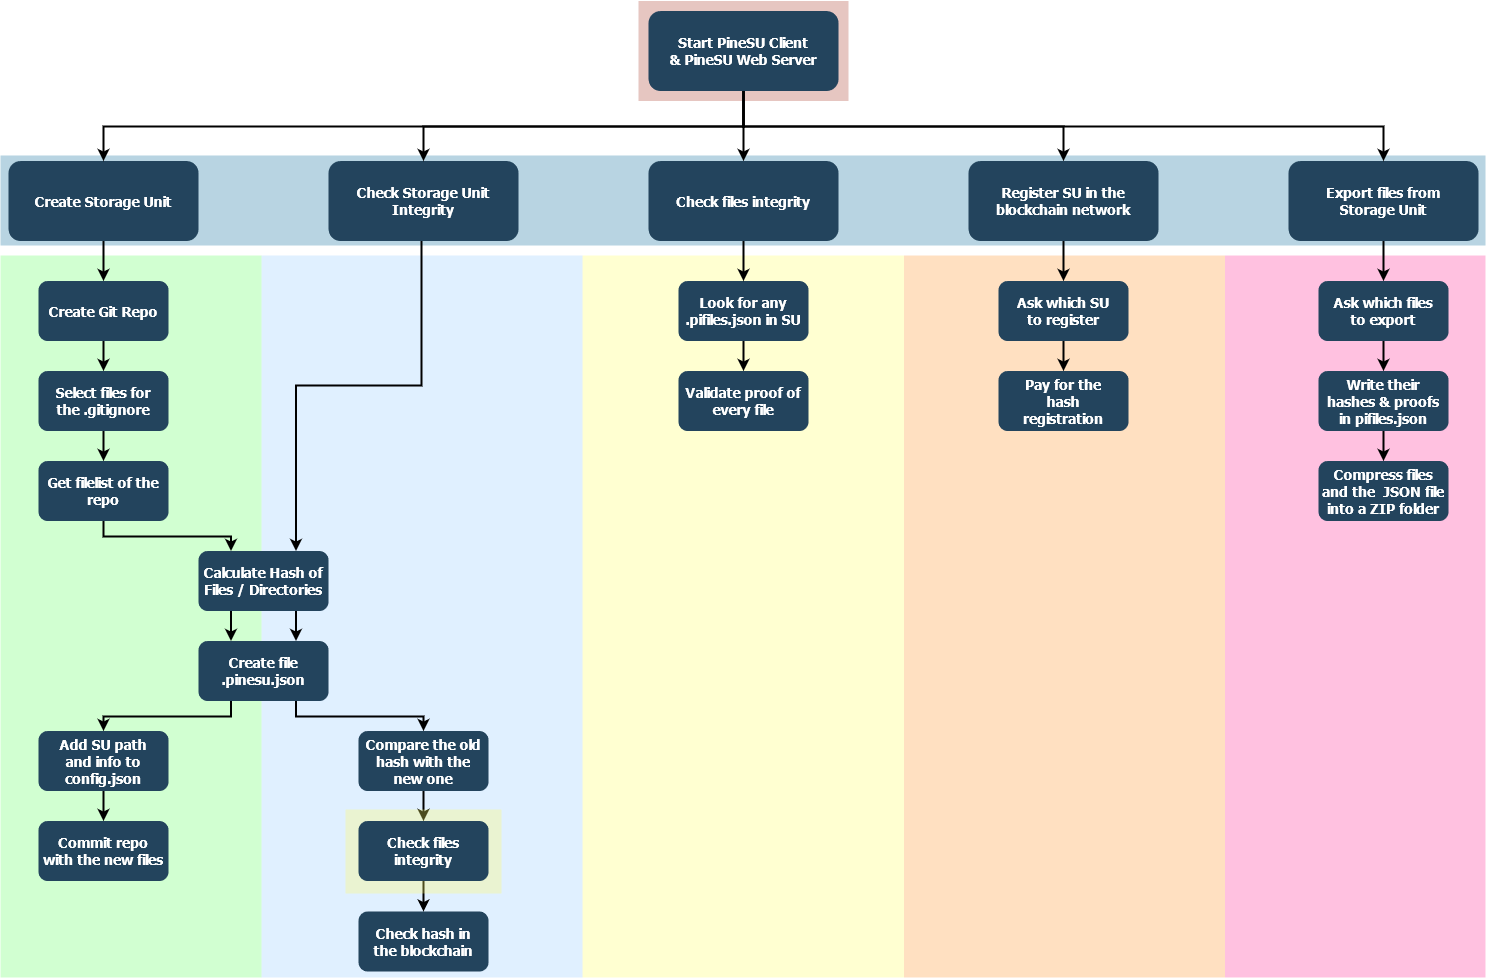
\includegraphics[width=1\textwidth]{figures/workflow.png}
	\end{figure}
\end{frame}
\begin{frame}
	\frametitle{Creazione del modulo di interrogazione e registrazione per la Blockchain}
	\begin{columns}
		\column{0.5\textwidth}
		\begin{figure}
			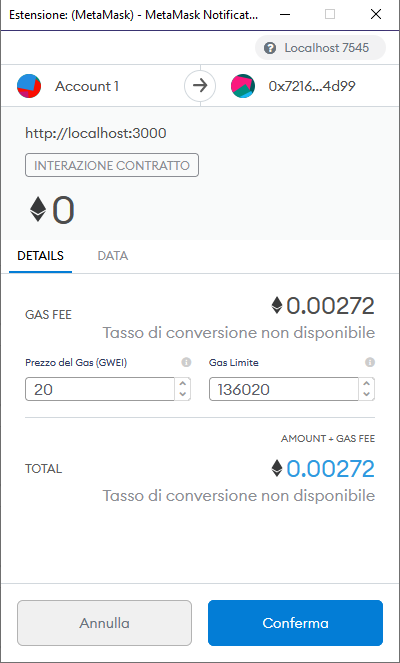
\includegraphics[width=0.6\textwidth]{figures/meta-gui.png}
			\caption{Transazione per registrare un hash nella blockchain}
		\end{figure}
		\column{0.5\textwidth}
		L’ultima parte della fase di implementazione è stata la realizzazione del Web Server locale che permette all’utente di registrare gli hash delle proprie Storage Unit nella blockchain, il risultato è stato ottenuto con una versione pesantemente modificata dell’applicazione \emph{sample} fornita dal sito della suite Truffle.
	\end{columns}
\end{frame}
\section{Resoconto}
\begin{frame}
	\frametitle{Resoconto}
	\begin{itemize}
		\item Data di inizio tirocinio: 15/2/2021
  		\item Data di fine tirocinio: 28/5/2021
  		\item Totale Ore: 150 (25 ore \(\cdot\) 6 CFU)
  		\item Professore Tutor: Luca Grilli
  		\item Studente Tirocinante: Paolo Speziali
  		\item Anno Accademico: 2020/2021
	\end{itemize}
\end{frame}
\section{Fonti}
\begin{frame}
	\frametitle{Fonti}
	\begin{itemize}
		\item \href{https://ethereum.org/it/developers/}{Strumenti Ethereum per sviluppatori} 
  		\item \href{https://www.trufflesuite.com/tutorial}{Tutorial Truffle DAPPs - Pet Shop}
  		\item \href{https://www.sitepoint.com/javascript-command-line-interface-cli-node-js/}{Build a JavaScript CLI with Node.js}
  		\item \href{https://developer.mozilla.org/en-US/docs/Learn/JavaScript/Asynchronous/Async_await}{Tutorial di Mozilla su async / await}
  		\item Immagini reperite dai siti ufficiali degli strumenti eccetto per alcune scaricate da queste pagine web:
			\begin{itemize}
				\item \href{https://www.poeticoding.com/hashing-a-file-in-elixir/}{Funzioni di Hashing}
				\item \href{https://www.romatoday.it/attualita/concorso-rai-fiera-roma-norme-covid-19.html}{Concorso pubblico}
				\item \href{https://www.criptovalute24.com/ethereum-migliora-la-sua-blockchain-rialzo-del-5-4/}{Ethereum Blockchain}
				\item \href{https://blog.netsons.com/git-software-guida-facile/}{Git repository}
				\item \href{https://amerlin.keantex.com/programmazione-asincrona-con-async-await-parte-2/}{async / await}
				\item \href{https://transparency.dev/verifiable-data-structures/}{Merkle Tree}
			\end{itemize}
			\item \href{https://waifu2x.booru.pics/Home/index}{Strumento di upscaling delle immagini} 
	\end{itemize}
\end{frame}
\end{document}